\documentclass[latex/main.tex]{subfiles}

\begin{document}
\section{Data Analysis}

\subsection{Dataset Description}\label{sec:dataset-description}

Resting fMRI (rfMRI) scans were provided by the Human Connectome Project (HCP), WU-Minn Consortium (led by principal investigators David Van Essen and Kamil Ugurbil; 1U54MH091657) funded by the 16 NIH Institutes and Centers supporting the NIH Blueprint for Neuroscience Research, and by the McDonnell Center for Systems Neuroscience at Washington University \citep{van_essen_wu-minn_2013}. Two subsets of the dataset were used: one for methods development and defining realistic simulation parameters (see \nameref{sec:simulations}), and the other for estimating high-resolution timescale maps of the cortex.\\

The \textit{methods development subset} included 10 subjects  (\#100004 - \#101410) scanned with a 3T gradient-echo EPI sequence (TR=720ms, slice thickness=2mm). Each subject completed four 15-minute runs (4800 timepoints total), preprocessed with standard steps including motion regression and artifact removal (see \citet{glasser_minimal_2013} for details). The resulting dataset dimensions were \{10 subjects, 4800 timepoints, 300 regions\}. The \textit{timescale mapping subset} included 180 subjects scanned with a 7T gradient-echo EPI sequence (TR=1000ms, slice thickness=1.6mm) over four 16-minute runs (3600 timepoints total), using the same preprocessing steps. Functional data were analyzed on the cortical surface down-sampled to 2mm spatial resolution, yielding a dataset with the dimensions \{180 subjects, 3600 timepoints, 64984 vertices\}. The time- and autocorrelation-domain methods were fit to each vertex independently, a mass-univariate analysis approach that resulted in subject-level maps of timescale estimates and their standard errors.\\

\subsubsection{Group-level Analysis}\label{sec:group-level-analysis}
Group-level maps combined individual timescales and standard errors, accounting for within- and between-subject variability. While remaining within the mass-univariate framework, for simplicity, we express the group timescale for the $N=180$ individual subjects at a single cortical vertex:
\begin{align}
    \hat\tau_n \; &\text{for} \; n\in\{1, 2, ..., N\}\\
    \hat\tau_N &= \frac{1}{N} \sum_{n=1}^N \hat\tau_n.
\end{align}

\noindent The group-level standard error for the timescale is given by the law of total variance:
\begin{align}
    \widehat{\text{se}}(\hat\tau_N) = \sqrt{\frac{1}{N} \sum_{n=1}^N \widehat{\text{se}}(\hat\tau_n)^2 + \frac{1}{N} \sum_{n=1}^N (\hat\tau_n - \hat\tau_N)^2}.
\end{align}

\noindent Here, the first term under the square root is the within-individual variance and the second term is the between-individual variance.\\

For visualization, brain-wide t-statistic maps tested whether timescales exceeded 0.5 seconds ($H_0: \tau \leq 0.5$) by the ratio:
\begin{align}\label{eq:t-ratio}
    t_N = \frac{\hat\tau_N-0.5}{\widehat{\text{se}}(\hat\tau_N)}.
\end{align}

\noindent Additionally, relative standard error (RSE) maps are presented to visualized the spatial precision of timescale estimates by the ratio:
\begin{align}
    \text{rse}(\hat\tau_N) = \frac{\widehat{\text{se}}(\hat\tau_N)}{\hat\tau_N}
\end{align}

\subsection{Data Analysis Results}
\begin{figure}[!ht]
    \centering
    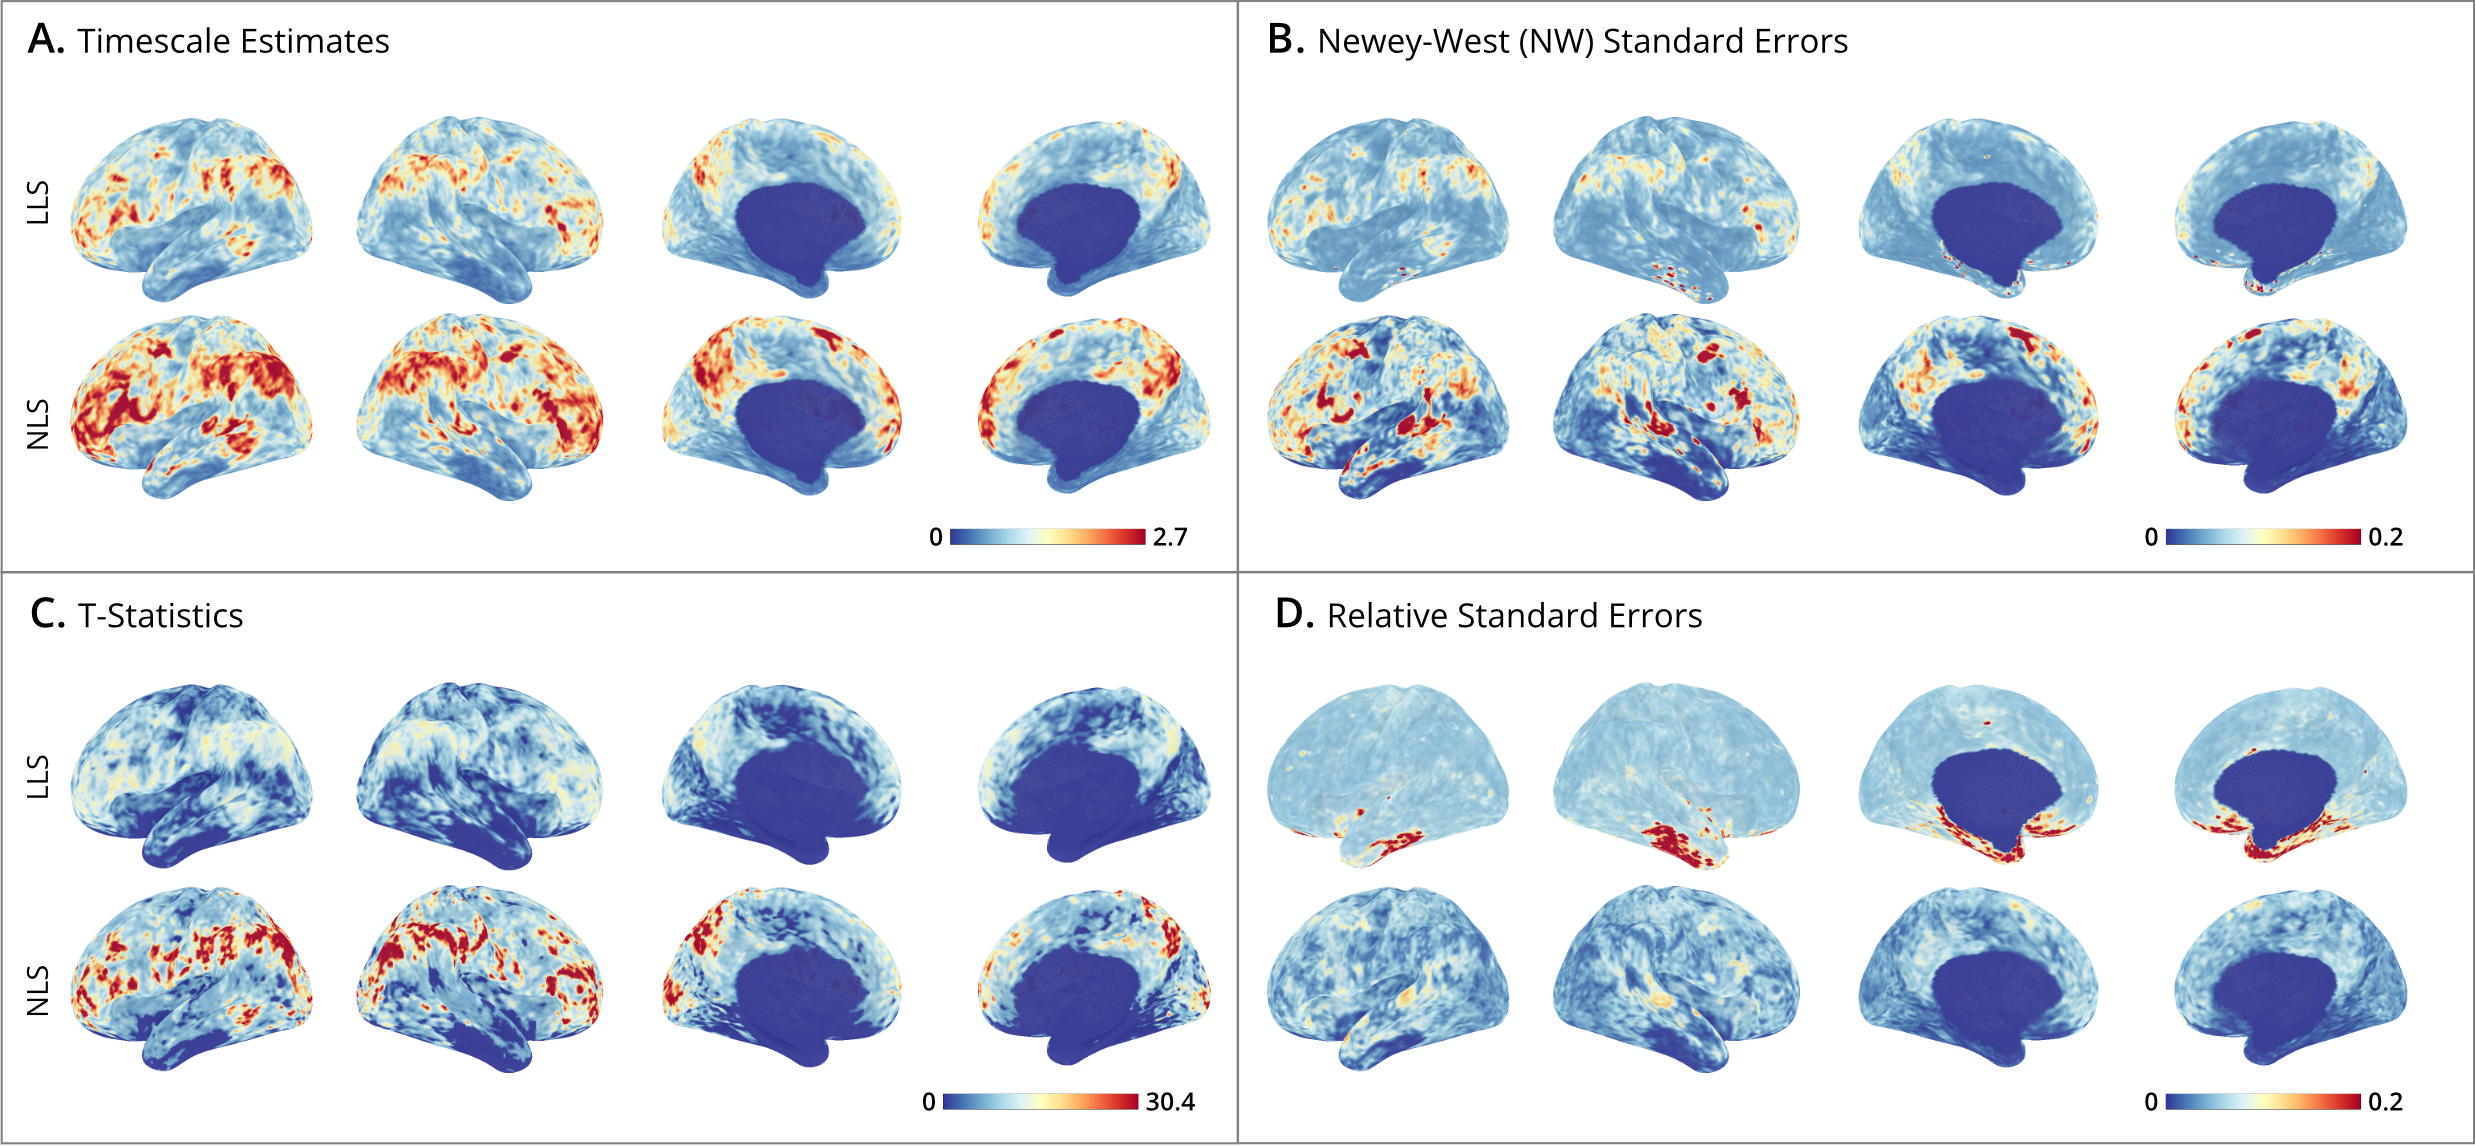
\includegraphics[width=1\textwidth]{figures/fig04-hcp1.png} 
    \caption{\textit{Human Connectome Project subject-level timescale maps.}}
    \subcaption*{
     (\textbf{A-D}) Cortical surface maps from HCP subject $\#100610$. Displays show lateral-left, lateral-right, medial-left, and medial-right views (excluding the medial wall). The upper bounds on the colorbars are set for each panel at the 99$^\text{th}$ percentile of cortical map values. For each panel, the top row shows results of the time-domain method (LLS), and the bottom row the autocorrelation-domain method (NLS). (\textbf{A}) Timescale estimates: maps display the timescales (in seconds) estimated at each vertex. (\textbf{B}) Newey-West standard errors: shows the spatial distribution of standard errors, where smaller values indicate greater estimation precision. (\textbf{B row 2}) shows the hybrid autocorrelation/time method.
     (\textbf{C}) T-statistics: unthresholded and uncorrected t-ratios testing where timescales exceed 0.5 seconds. (\textbf{D}) Relative Standard Errors (RSEs): relative reliability of estimates, where low RSE (near zero) indicates high precision with small uncertainty.
    }
    \label{fig:map-hcp1}
\end{figure}

\begin{figure}[!ht]
    \centering
    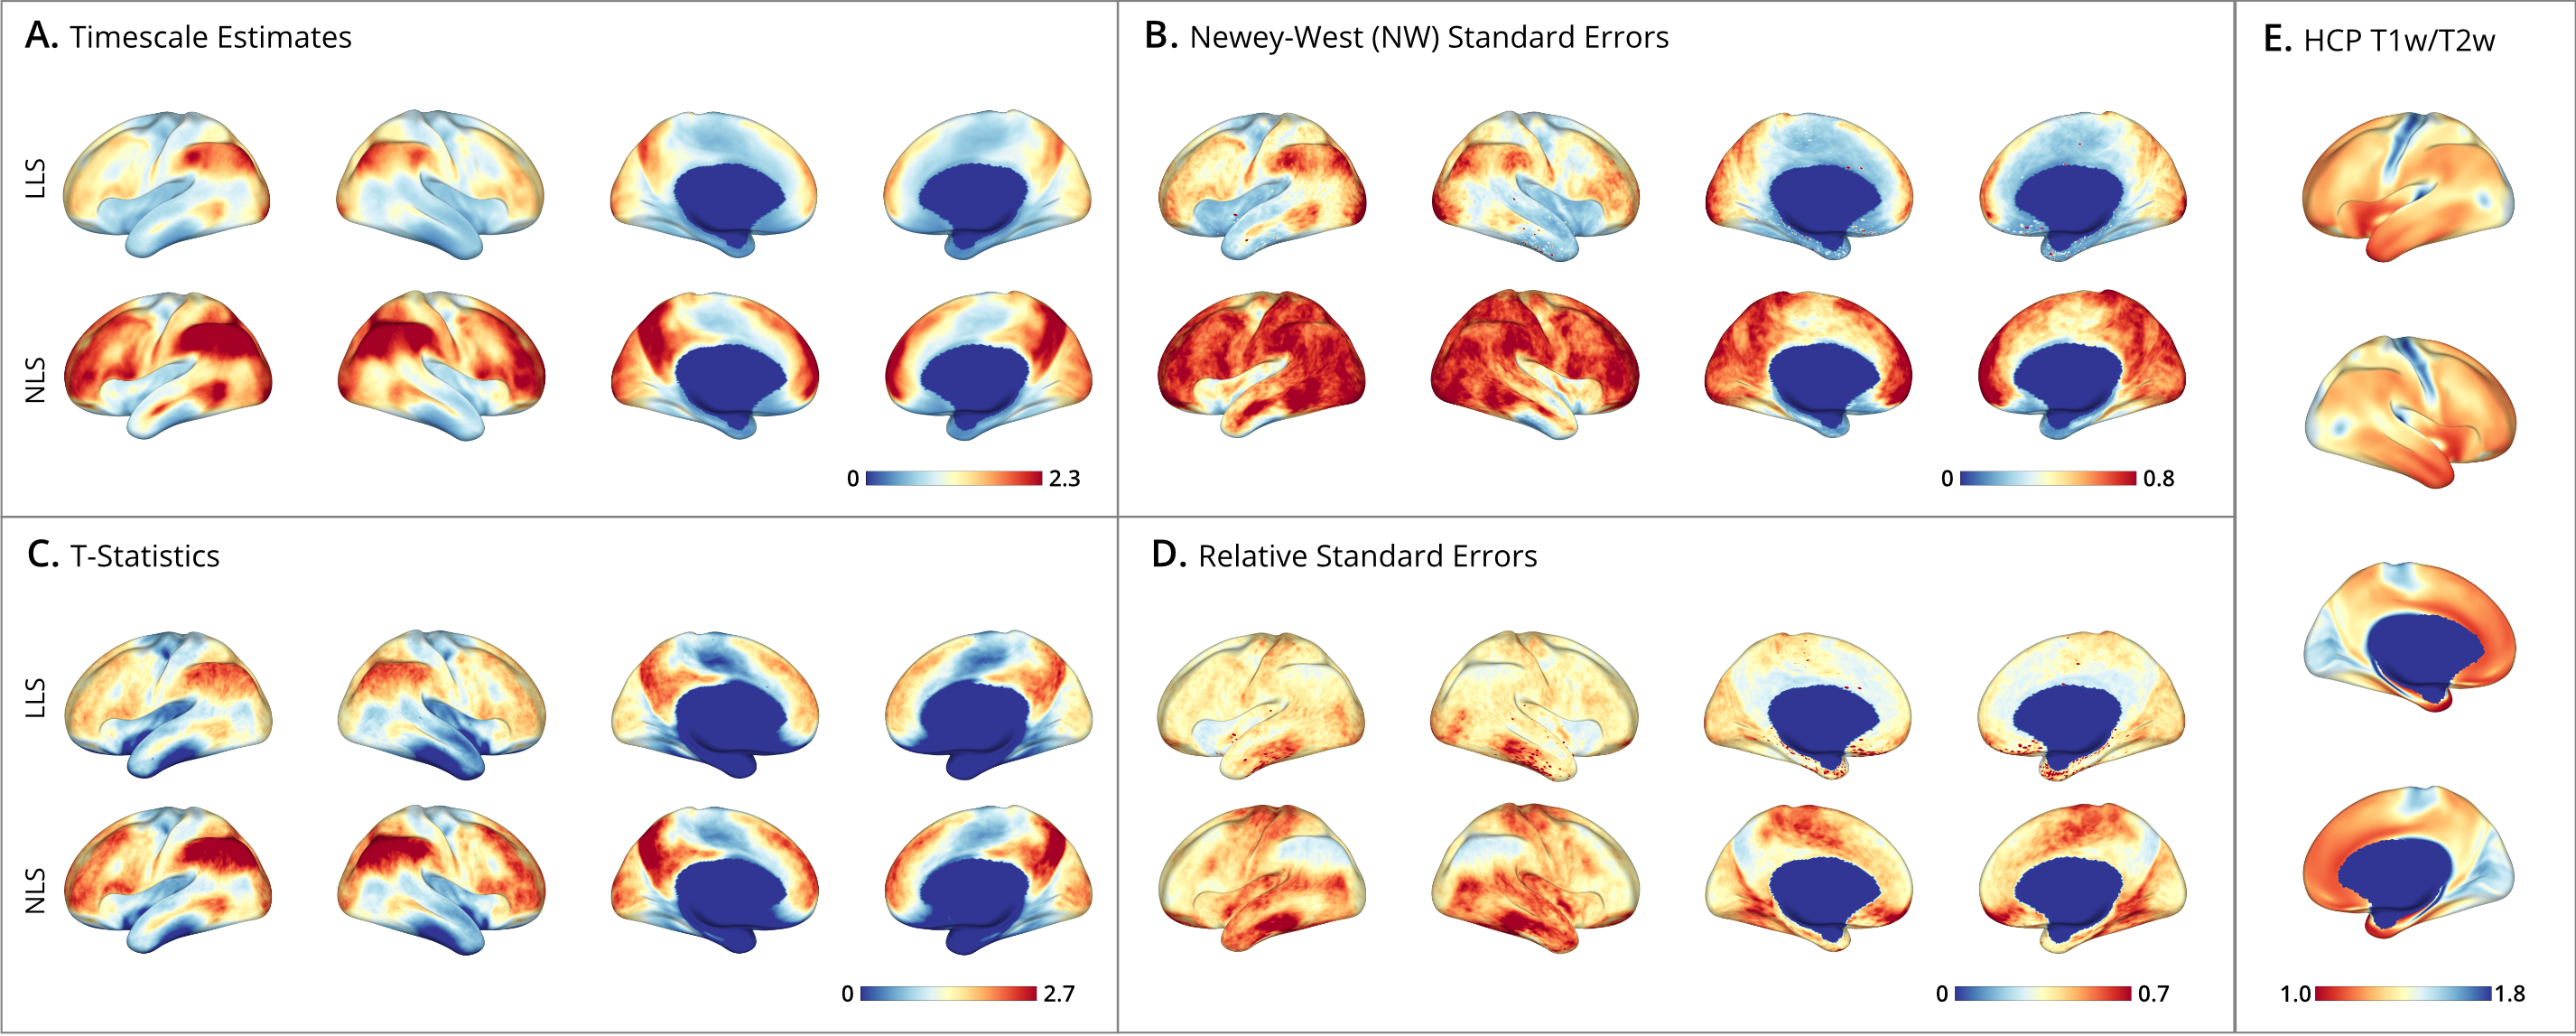
\includegraphics[width=1\textwidth]{figures/fig05-hcp180.png} 
    \caption{\textit{Human Connectome Project group-level timescale maps.}}
    \subcaption*{
    (\textbf{A-D}) Cortical surface maps from $N=180$ HCP subjects. Displays show lateral-left, lateral-right, medial-left, and medial-right views (excluding the medial wall). The upper bounds on the colorbars are set for each panel at the 99$^\text{th}$ percentile of cortical map values. For each panel, the top row shows results of the time-domain method (LLS), and the bottom row the autocorrelation-domain method (NLS).
    (\textbf{A}) Timescale estimates: maps display the group-level timescales (in seconds) at each vertex, averaged over subjects.
    (\textbf{B}) Newey-West standard errors: group-level spatial distribution of estimates, accounting for within- and between-subject variability. Smaller values indicate greater precision.
    (\textbf{C}) T-statistics: unthresholded and uncorrected t-ratios testing where group-level timescales exceed 0.5 seconds.
    (\textbf{D}) Relative standard errors (RSEs): relative reliability of estimates, where low RSE (near zero) indicates high precision with small uncertainty across subjects.
    (\textbf{E}) Timescale organization by brain network: maps display brain networks from the Yeo 7 Network Atlas, ordered by the network-averaged t-statistics (from panel C). This ordering is the same for LLS and NLS methods, and highlights the hierarchical organization of timescales, progressing from sensory networks (e.g., somatomotor and limbic in blues) to association networks (e.g., frontoparietal and default mode in reds).
    }
    \label{fig:map-hcp180}
\end{figure}

\subsubsection{Results for rfMRI Timescale Maps}
Subject-level maps were generated by mass-univariate fitting of LLS and NLS estimators to cortical surface data. \textbf{Panel A} presents the spatial distribution of timescale estimates, which show that NLS estimates tend to yield larger timescales than LLS, consistent with simulation results. \textbf{Panel B} shows the corresponding maps of standard errors, which appear align with the timescale maps, consistent with the simulation finding that larger timescales are associated with greater sampling variability. \textbf{Panel C} depicts the relative ratio of timescale estimates to their standard errors (i.e., t-statistics), testing whether the timescales significantly exceed a half second ($H_0: \tau \leq 0.5$). Despite larger standard errors for higher timescales, these regions still exhibit higher t-statistics. \textbf{Panel D} shows low RSEs across much of the brain indicating high estimation reliability. \\

Group-level timescale maps were generated by combining individual estimates to account for both within-individual and between-individual variability, providing an aggregate view of timescale distributions across subjects. \textbf{Panel A} shows that the average timescale maps for both LLS and NLS estimators are smoother than the individual maps, displaying a well-organized spatial pattern across the cortex, with NLS estimates generally being larger than LLS. \textbf{Panel B} presents the standard error maps, which combine variances from within-subject Newey-West estimates and between-subject timescale estimates. As expected from the simulation results, the standard errors are larger for NLS than for LLS. \textbf{Panel C} depicts t-statistics testing whether timescales exceed a half second, showing that both methods yield comparable results. \textbf{Panel D} plots relative standard errors (RSEs), illustrating the general trend that regions with larger timescales are easier to estimate, while areas with smaller timescales exhibit greater uncertainty. This is particularly apparent in the limbic network comprising orbital frontal cortex and anterior temporal cortex. \textbf{Panel E} highlights the spatial organization of timescales into networks, by mapping the t-statistic at each vertex to one of seven networks from the \citet{thomas_yeo_organization_2011} atlas. The ordering \{limbic, somatomotor, ventral attention, visual, dorsal attention, default, frontoparietal\} aligns with the sensory-to-association axis of brain organization, and is consistent with a large literature on the hierarchical organization of timescales \citep{murray_hierarchy_2014, hasson_hierarchy_2008, stephens_place_2013, raut_hierarchical_2020, gao_neuronal_2020, hasson_hierarchy_2008}. Sensory networks (limbic and somatomotor) have short timescales, followed by attentional networks (ventral and dorsal attention), and finally higher-order association networks (default mode and frontoparietal) contain the largest timescales.\\ 

This empirical analysis highlights methodological considerations for estimating fMRI timescale maps. (1) Both time-domain (LLS) and autocorrelation-domain (NLS) methods produce similar maps, but diverge at extremes -- NLS yields larger timescales. The corresponding standard errors for NLS are also larger, so the resulting t-ratio maps remain similar between the two methods, highlighting why point estimates can be misleading without considering standard errors.  Likewise, estimates are on average more precise for LLS, consistent with simulation results.  (2) In this mass-univariate analysis, the computational cost of LLS is substantially lower than NLS because of its simple analytical solution. (3) The t-statistic maps organized by brain network exhibit a clear hierarchical timescale organization, reflecting how networks integrate and process information over time. And this pattern is consistent regardless of the estimation method. Taken together, these findings suggest that time-domain method may be preferable for large-scale neuroimaging studies due to its computational efficiency and higher precision, while producing maps consistent with previously reported timescale hierarchies. 
\end{document}